\subsection{Sprint Planning}\labelssec{sp4:planning}

Se precedentemente è stato realizzato il sistema come concentrato, in questo Sprint l'obiettivo è realizzare un sistema distribuito in grado di soddisfare il committente.

Al termine di questo Sprint si vuole avere un sistema in grado di eseguire la logica del robot su un robot fisico e la console su una differente macchina;
deve essere possibile controllare il robot secondo le specifiche fornite con i requisiti, avendo il comportamento atteso.

In particolare, il focus di questo Sprint è sui seguenti 3 punti:

\begin{itemize}
  \item
    miglioramento della gestione dell'ostacolo del robot \requirementref{discovery}
    e implementazione della logica di recupero del robot \requirementref{retriever};
  \item
    realizzazione del robot fisico;
  \item
    distribuzione del sistema tra robot fisico e \requirementref{console}.
\end{itemize}

\subsection{Analisi dei requisiti}\labelssec{sp4:req_analysis}

Dopo aver definito l'obiettivo di massima di questo Sprint, si è proceduto con l'individuazione dei requisiti specifici da realizzare:

\begin{description}
  \item[\requirementref{R-takePhoto}]:
    il robot deve scattare una fotografia all'ostacolo appena individuato.

  \item[\requirementref{R-sendPhoto}]:
    il robot deve inviare la fotografia appena scattata alla console.

  \item[\requirementref{R-storePhoto}]:
    se la fotografia ricevuta dalla console rappresenta un ostacolo classificato come bomba deve essere salvata
    in modo permanente contestualmente alle informazioni relative.
    Le informazione in questione sono la posizione della bomba e il tempo alla rilevazione della bomba.

    Non viene specificato quale debba essere la modalità e la posizione di salvataggio.
    Il committente fornisce però libertà su questo.

  \item[\requirementref{R-waitForHome}]:
    il sistema deve attendere che il robot \requirementref{discovery} torni alla base, in una condizione che non consenta di effettuare alcuna azione.

  \item[\requirementref{R-reachBag}]:
    il robot \requirementref{retriever} deve raggiungere la posizione dell'ordigno indicata nella mappa,
    ottimizzando il percorso al fine di evitare ostacoli già rilevati dal robot \requirementref{discovery}.

    L'assunzione fatta è che il territorio sia rimasto invariato rispetto alla fase di esplorazione precedente.

  \item[\requirementref{R-bagAtHome}]:
    il robot \requirementref{retriever} dopo aver raccolto l’ordigno in un contenitore sicuro deve tornare alla base,
    evitando gli ostacoli come in precedenza.

\end{description}

\subsection{Analisi del problema}\labelssec{sp4:prob_analysis}

A seguito dell'analisi dei requisiti, sono state fatte diverse considerazioni sui problemi emersi;
di seguito si descrive nel dettaglio ciascuna di queste.

\subsubsection{Robot retriever}\labelsssec{sp4:retriever}

Analizzando il comportamento che dovrebbe tenere il robot retriever e le interazioni previste, risulta evidente che possano essere utilizzati gli stessi strumenti a disposizione del robot discovery (come ad esempio il planner, il robot advanced, ecc\ldots);
la principale differenza al riguardo è che il retriever non deve esplorare la hall, ma deve essere dotato di conoscenza della mappa prima ancora di partire.

Il presupposto è che il robot non debba mai incontrare ostacoli se non quando giunge alla bomba (\requirementref{R-reachBag}), caso in cui la carica e torna a casa (\requirementref{R-bagAtHome}).

\subsubsection{Condivisione dello stato della temperatura}

Il committente non ha espresso particolari requisiti a riguardo di come viene recuperata l'informazione sulla temperatura;
durante la fase di analisi, si è deciso di fornire la massima elasticità al sistema, veicolando questa informazione tramite un evento su MQTT\@.

\begin{figure}[H]
  \centering
  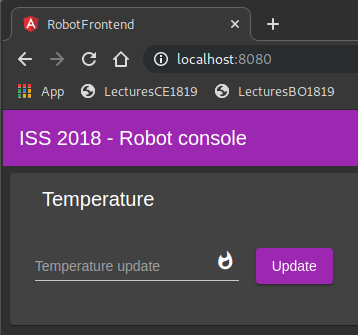
\includegraphics[width=0.35\textwidth]{res/sprint4/temp-ctrl.png}%
  \label{fig:sp4:temp-ctrl}
\end{figure}

La soluzione più semplice è risultata la realizzazione di un servizio che emette questa informazione a comando dell'utente:
per rendere più user-friendly questa funzionalità, si è scelto di integrare il controllo della temperatura nell'interfaccia grafica già presente.

\subsubsection{Dotazione della fotocamera}\labelsssec{sp4:camera}

Da requisiti il committente ha richiesto che quando si incontra un ostacolo (\requirementref{R-stopAtBag}), il robot discovery deve inviare alla console un'immagine di quest'ultimo (\requirementref{R-takePhoto} e \requirementref{R-sendPhoto}).

Dato che tra le componenti in possesso in questa fase non è presente una fotocamera, per poter comunque mostrare il corretto funzionamento del sistema al committente si è deciso di emulare la fotocamera precaricando delle immagini nel robot.

\subsubsection{Informazioni aggiuntive sullo stato}

Oltre alle informazioni di base dello stato del sistema si è mostrato necessario trasmettere all'interfaccia grafica anche altre informazioni, come un avviso nel caso in cui la temperatura salga sopra la soglia fissata o l'immagine dell'ostacolo per permettere all'utente di riconoscere la bomba (\requirementref{R-sendPhoto});
per questa ragione è importante analizzare il problema di come veicolare lo scambio di queste informazioni dal sistema all'interfaccia.

A tale proposito, nessuno dei requisiti utente impone alcuna scelta, dunque si è deciso di procedere con l'approccio più semplice e riutilizzabile:
aggiungere queste informazioni allo stato che la console invia periodicamente alle interfacce grafiche.

Questo approccio, unito al fatto che è la console stessa a specificare all'interno dello stato quali azioni sono possibili, abilita alla possibilità di inviare messaggi con azioni custom nel caso in cui in futuro ciò si dimostri necessario.

\subsubsection{Storage foto}

Da requisiti concordati con il committente, è necessario memorizzare la foto della bomba incontrata (\requirementref{R-storePhoto}).

A tale proposito sono state pensate due possibili approcci alla memorizzazione:

\begin{enumerate}
  \item allegare la foto della bomba al messaggio di risposta dal front-end alla console, dove viene poi salvata permanentemente;
  \item memorizzare temporaneamente sulla console l'ultima foto scattata e nel caso l'operatore segnali la presenza della bomba, salvarla su uno storage permanente.
\end{enumerate}

Dato che non è stata fatta alcuna richiesta dal committente, si è deciso di ottimizzare i dati scambiati attraverso la rete, scegliendo la seconda soluzione, dove l'immagine viene inviata una sola volta per ostacolo.

Per quanto riguarda lo storage sul quale memorizzare tali foto (\requirementref{R-storePhoto}), si richiede di memorizzare l'immagine assieme ad alcune informazioni di contesto:
in pratica lo stato per come lo conosce la console.

La memorizzazione di tali foto può essere fatta sia in localmente al robot, che in remoto, per esempio sulla console o un servizio esterno.
Dato che il robot è in possesso della sola foto e non delle informazioni di contesto, è illogico memorizzare tale foto sul robot.
Per quanto riguarda la memorizzazione su console o servizio remoto, il committente non ha espresso preferenze a riguardo, perciò ancora una volta è stata scelta la soluzione più semplice:
memorizzare su file nella console.

\subsubsection{Condivisione della mappa}

Nel momento in cui si aggiunge il robot retriever al sistema, è necessario discutere il problema della condivisione della mappa;
fino a questo momento, si era considerata solamente l'esplorazione del robot discovery e la mappa era memorizzata internamente a questo e notificata alla console solamente per permetterne la visualizzazione nel front-end.

Aggiungendo il robot retriever, invece, si è ritenuto utile che al suo avvio gli venga condivisa la mappa in modo da iniziare il suo lavoro avendo già questa nella sua base di conoscenza.
Per condividere questa informazione si è scelto di utilizzare un messaggio, in quanto si vuole solamente che il robot retriever venga notificato della mappa.

In particolare, si hanno due possibili soluzioni:

\begin{enumerate}
  \item il robot discovery invia tale informazione al robot retriever;
  \item la console notifica il robot retriever di tale informazione.
\end{enumerate}

Si è scelto di seguire la seconda strada: sarà dunque la console, come punto di controllo centrale, a tenere la rappresentazione corrente della mappa e a notificare il retriever.
Si è preferito questo alla prima strada in quanto avrebbe altrimenti forzato nel sistema un vincolo troppo restrittivo per il quale il robot discovery ed il retriever devono essere presenti entrambi all'avvio del secondo.

\subsubsection{Robot hardware}

Per quanto ne fosse stata mantenuta la compatibilità fin dall'inizio, negli Sprint precedenti si era sempre evitato di ragionare sulla componente hardware del sistema.

In questo ultimo Sprint, invece, nella fase di analisi si è anche ragionato sullo schema da utilizzare per la costruzione di un robot semovente in grado di eseguire il codice finora realizzato.

\begin{figure}[H]
  \centering
  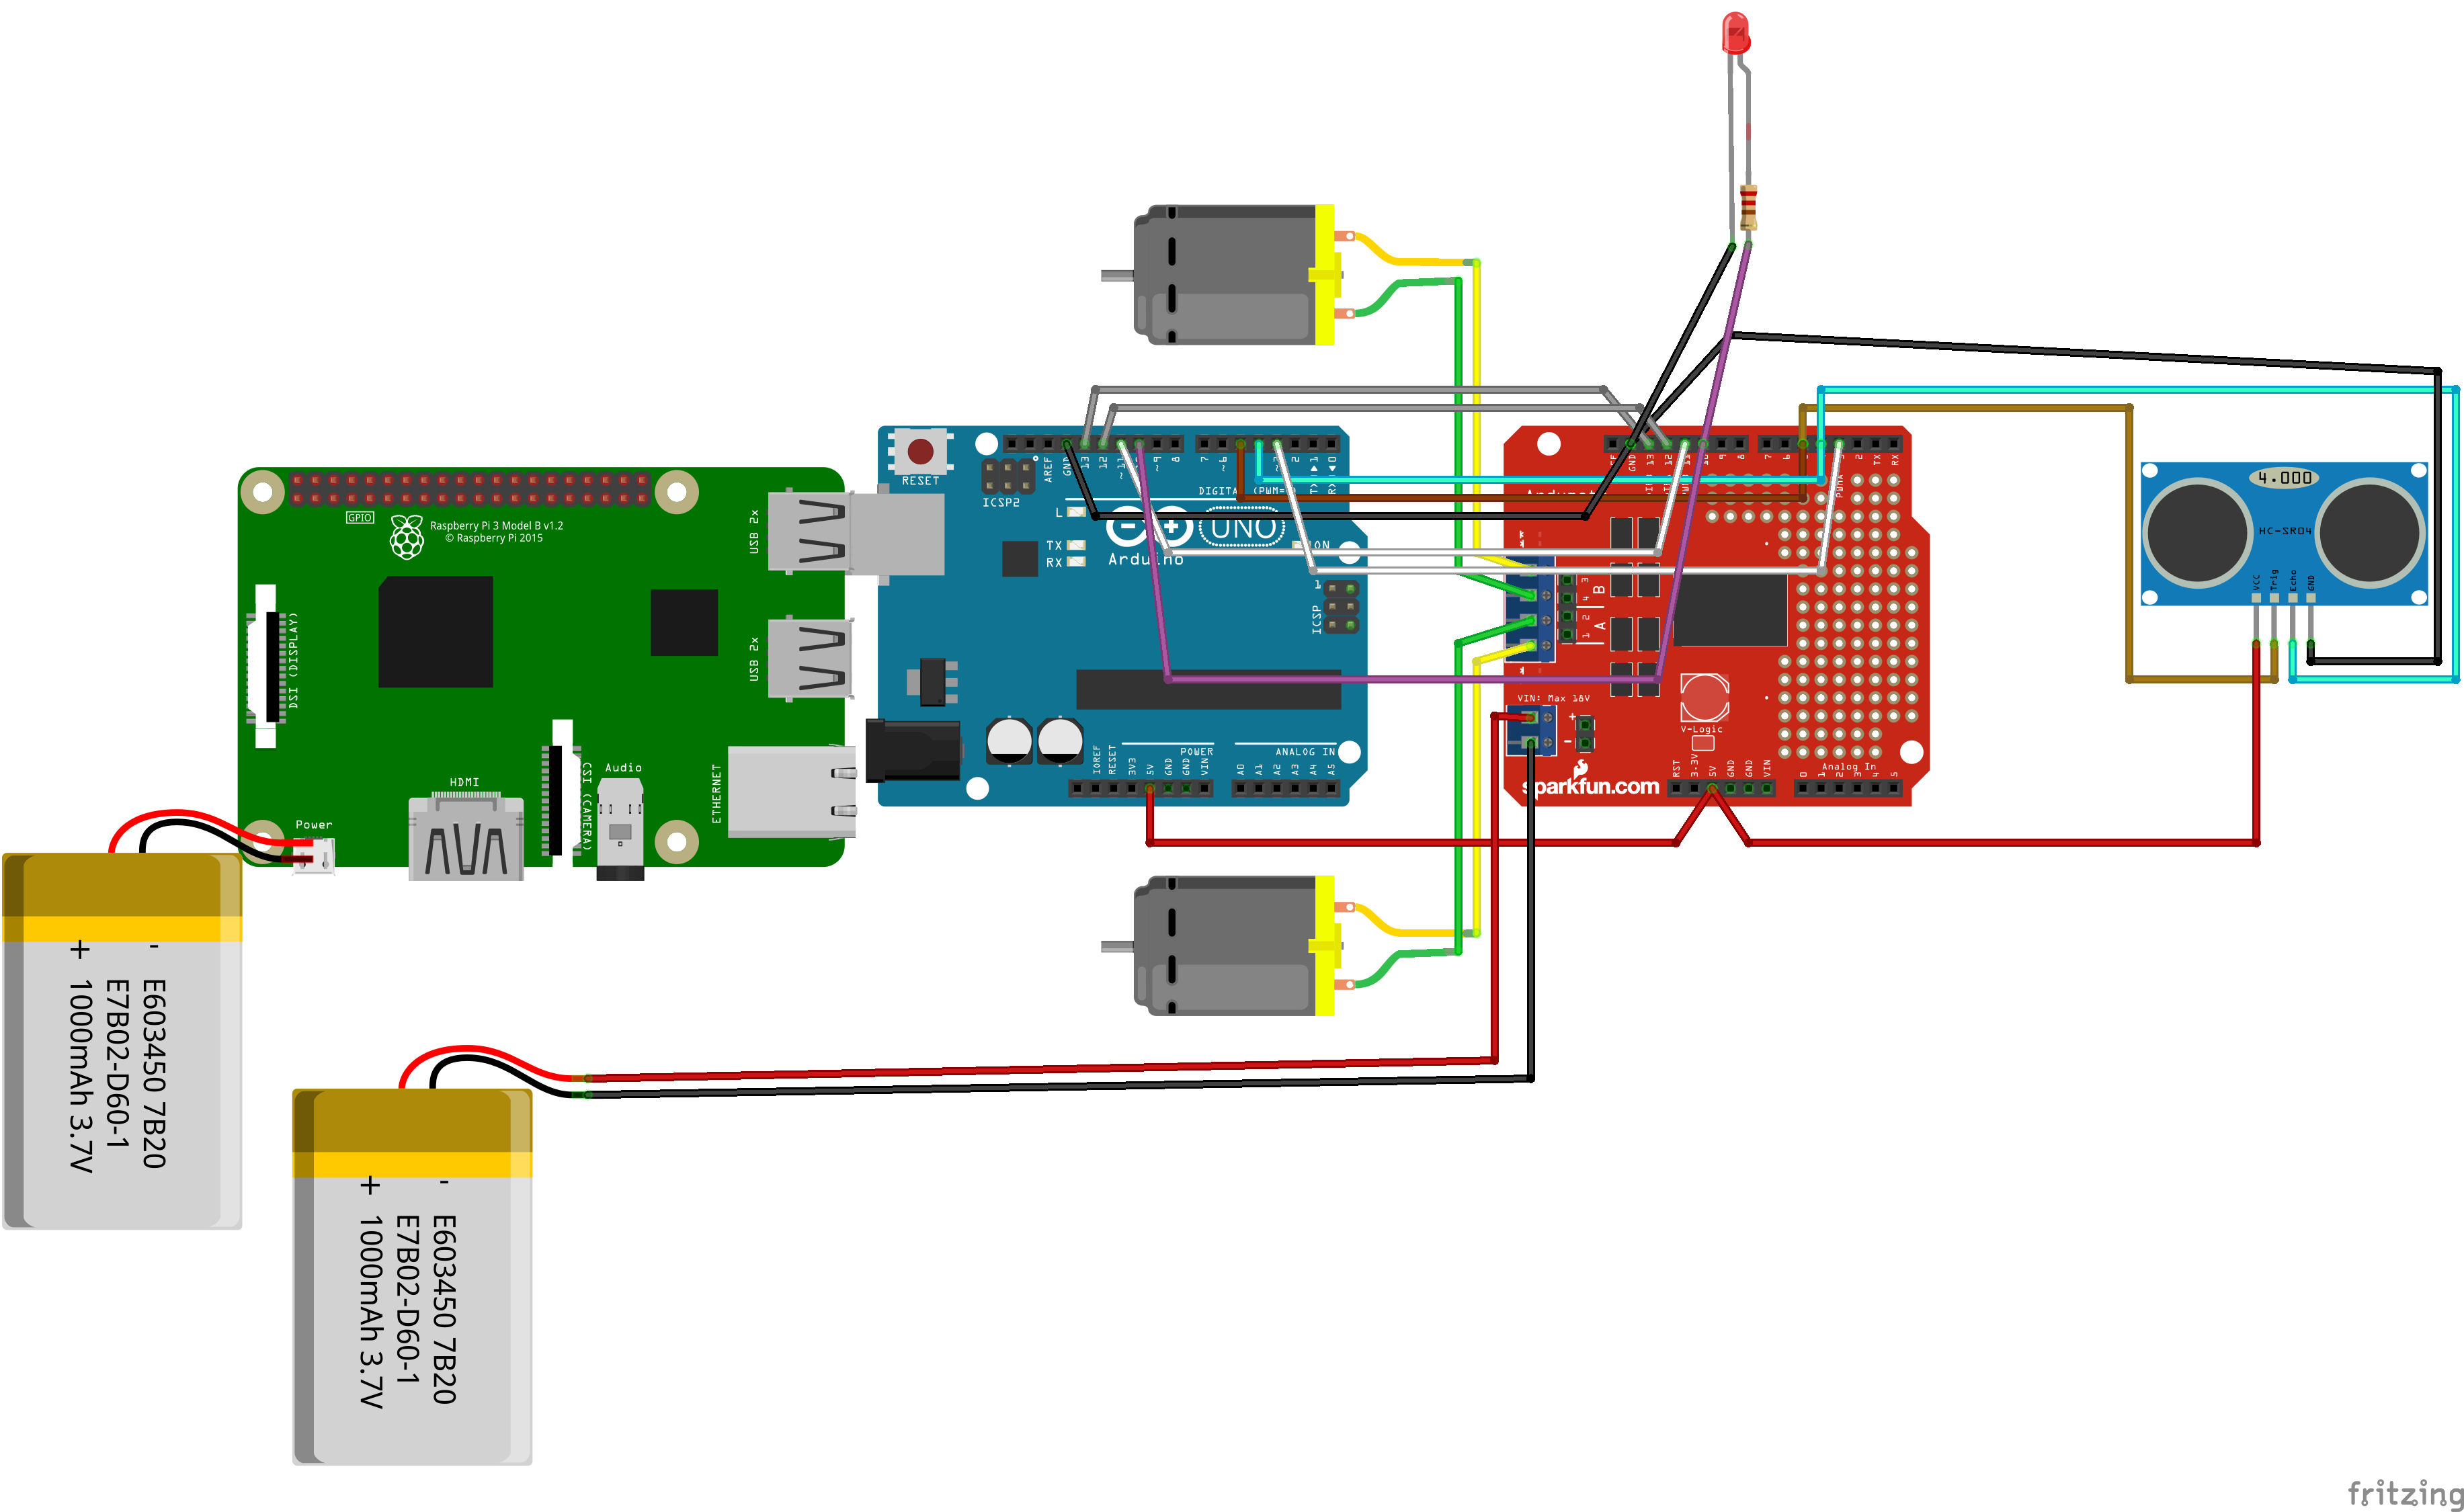
\includegraphics[width=0.9\textwidth]{res/sprint4/NanoBotArduino.png}%
  \caption{Rappresentazione schematica delle connessioni tra i dispositivi HW}%
  \label{fig:sp4:nanobot}
\end{figure}

Come è possibile vedere in \Cref{fig:sp4:nanobot}, il sistema è composto da due SoC principali:

\begin{itemize}
  \item
    un Raspberry Pi 3, in grado di eseguire Linux e il codice Java realizzato;
    esso è inoltre in grado di collegarsi alla rete per servire l'interfaccia web con cui interagire con il sistema.
  \item
    un Arduino Uno, connesso tramite seriale via USB al Raspberry Pi e tramite GPIO ai seguenti componenti:
    \begin{itemize}
      \item uno shield con un ponte H per pilotare i due motori;
      \item un LED\@;
      \item un sensore di prossimità a ultrasuoni (HC-SR04).
    \end{itemize}
\end{itemize}

Sul robot sono montate due pacchi batteria al litio, uno per ciascuna delle componenti principali.

\subsubsection{Da locale a distribuito}

Durante questo Sprint, si è andati a delocalizzare la soluzione separando il sistema in due nodi principali:
il robot e la console.

Il contesto del robot contiene non solo tutta la gestione del robot (robot-adapter, robot-advanced, \ldots), ma anche la business logic del suo funzionamento (le due mind).

Il contesto della console contiene naturalmente la console, ma anche il world-observer.
Non ha infatti senso alcuno sovraccaricare il robot, già sensibile, con l'elaborazione di tutti gli input esterni sulle condizioni dell'environment.

\begin{figure}[H]
  \centering
  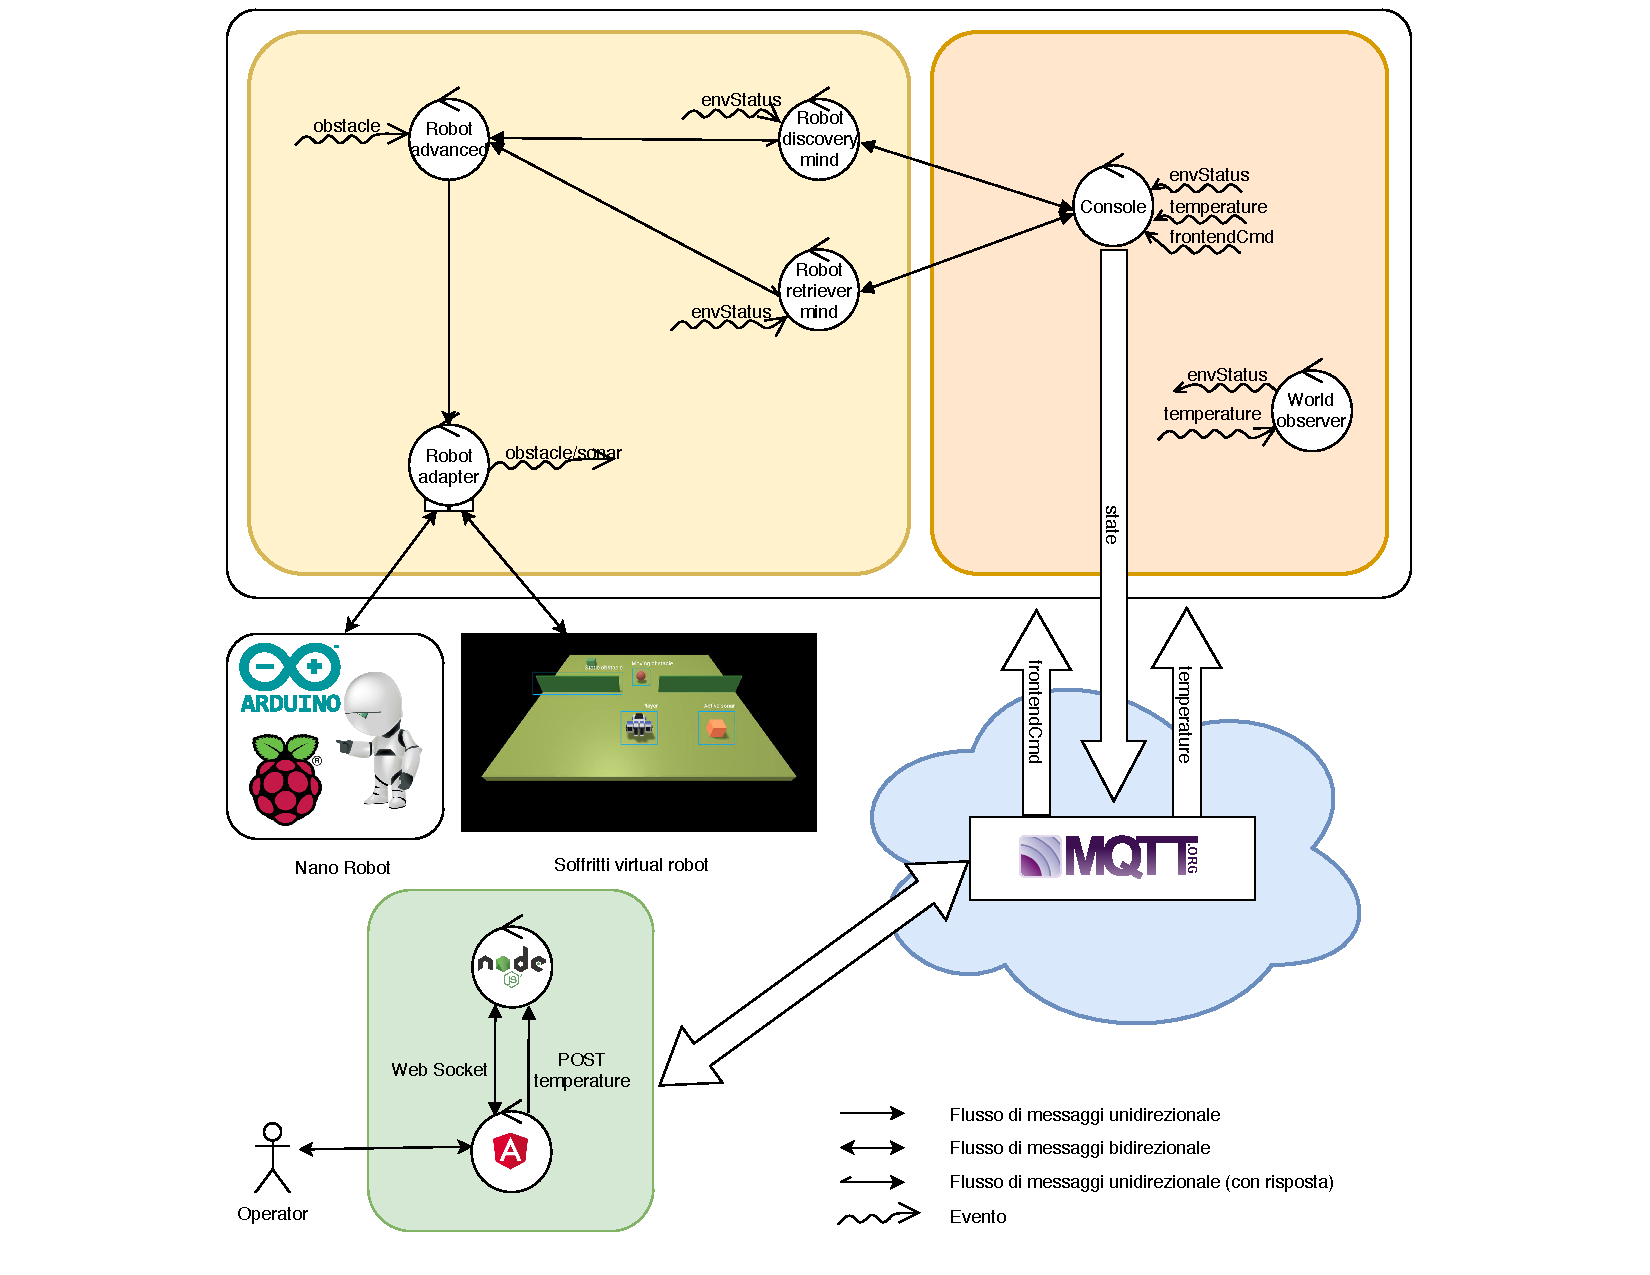
\includegraphics[width=0.9\textwidth]{res/system.pdf}%
  \caption{Schema globale del sistema sviluppato con informazioni dettagliate}%
  \label{fig:sp4:system}
\end{figure}

Il sistema distribuito eterogeneo risultante è quello rappresentato in~\Cref{fig:sp4:system}.

\subsection{Progettazione}\labelssec{sp4:project}

\subsubsection{Arduino e PlatformIO}

Per la realizzazione del codice alla base del robot fisico, si è deciso di partire da codice già presente all'interno della software house, opportunamente adattato a build system più moderni.
In particolare, la software house metteva a disposizione soprattutto codice pensato per l'utilizzo con l'mBot\footnote{\url{https://www.makeblock.com/steam-kits/mbot}} prodotto da Makeblock, hardware giudicato purtroppo troppo costoso per gli obiettivi del progetto.
In alternativa, era fornito anche codice per robot Arduino custom; si è deciso dunque di partire da questo codice, sostituendo il build system della toolchain di Arduino con PlatformIO\footnote{\url{https://platformio.org/}}.

Questa scelta ha permesso, innanzitutto, di configurare il provider di continuous integration di eseguire build del codice ad ogni push sul repository GitHub utilizzato;
inoltre, la toolchain messa a disposizione è molto flessibile e può essere utilizzata per il debug anche in modalità headless su Raspberry Pi.

\begin{figure}[H]
  \centering
  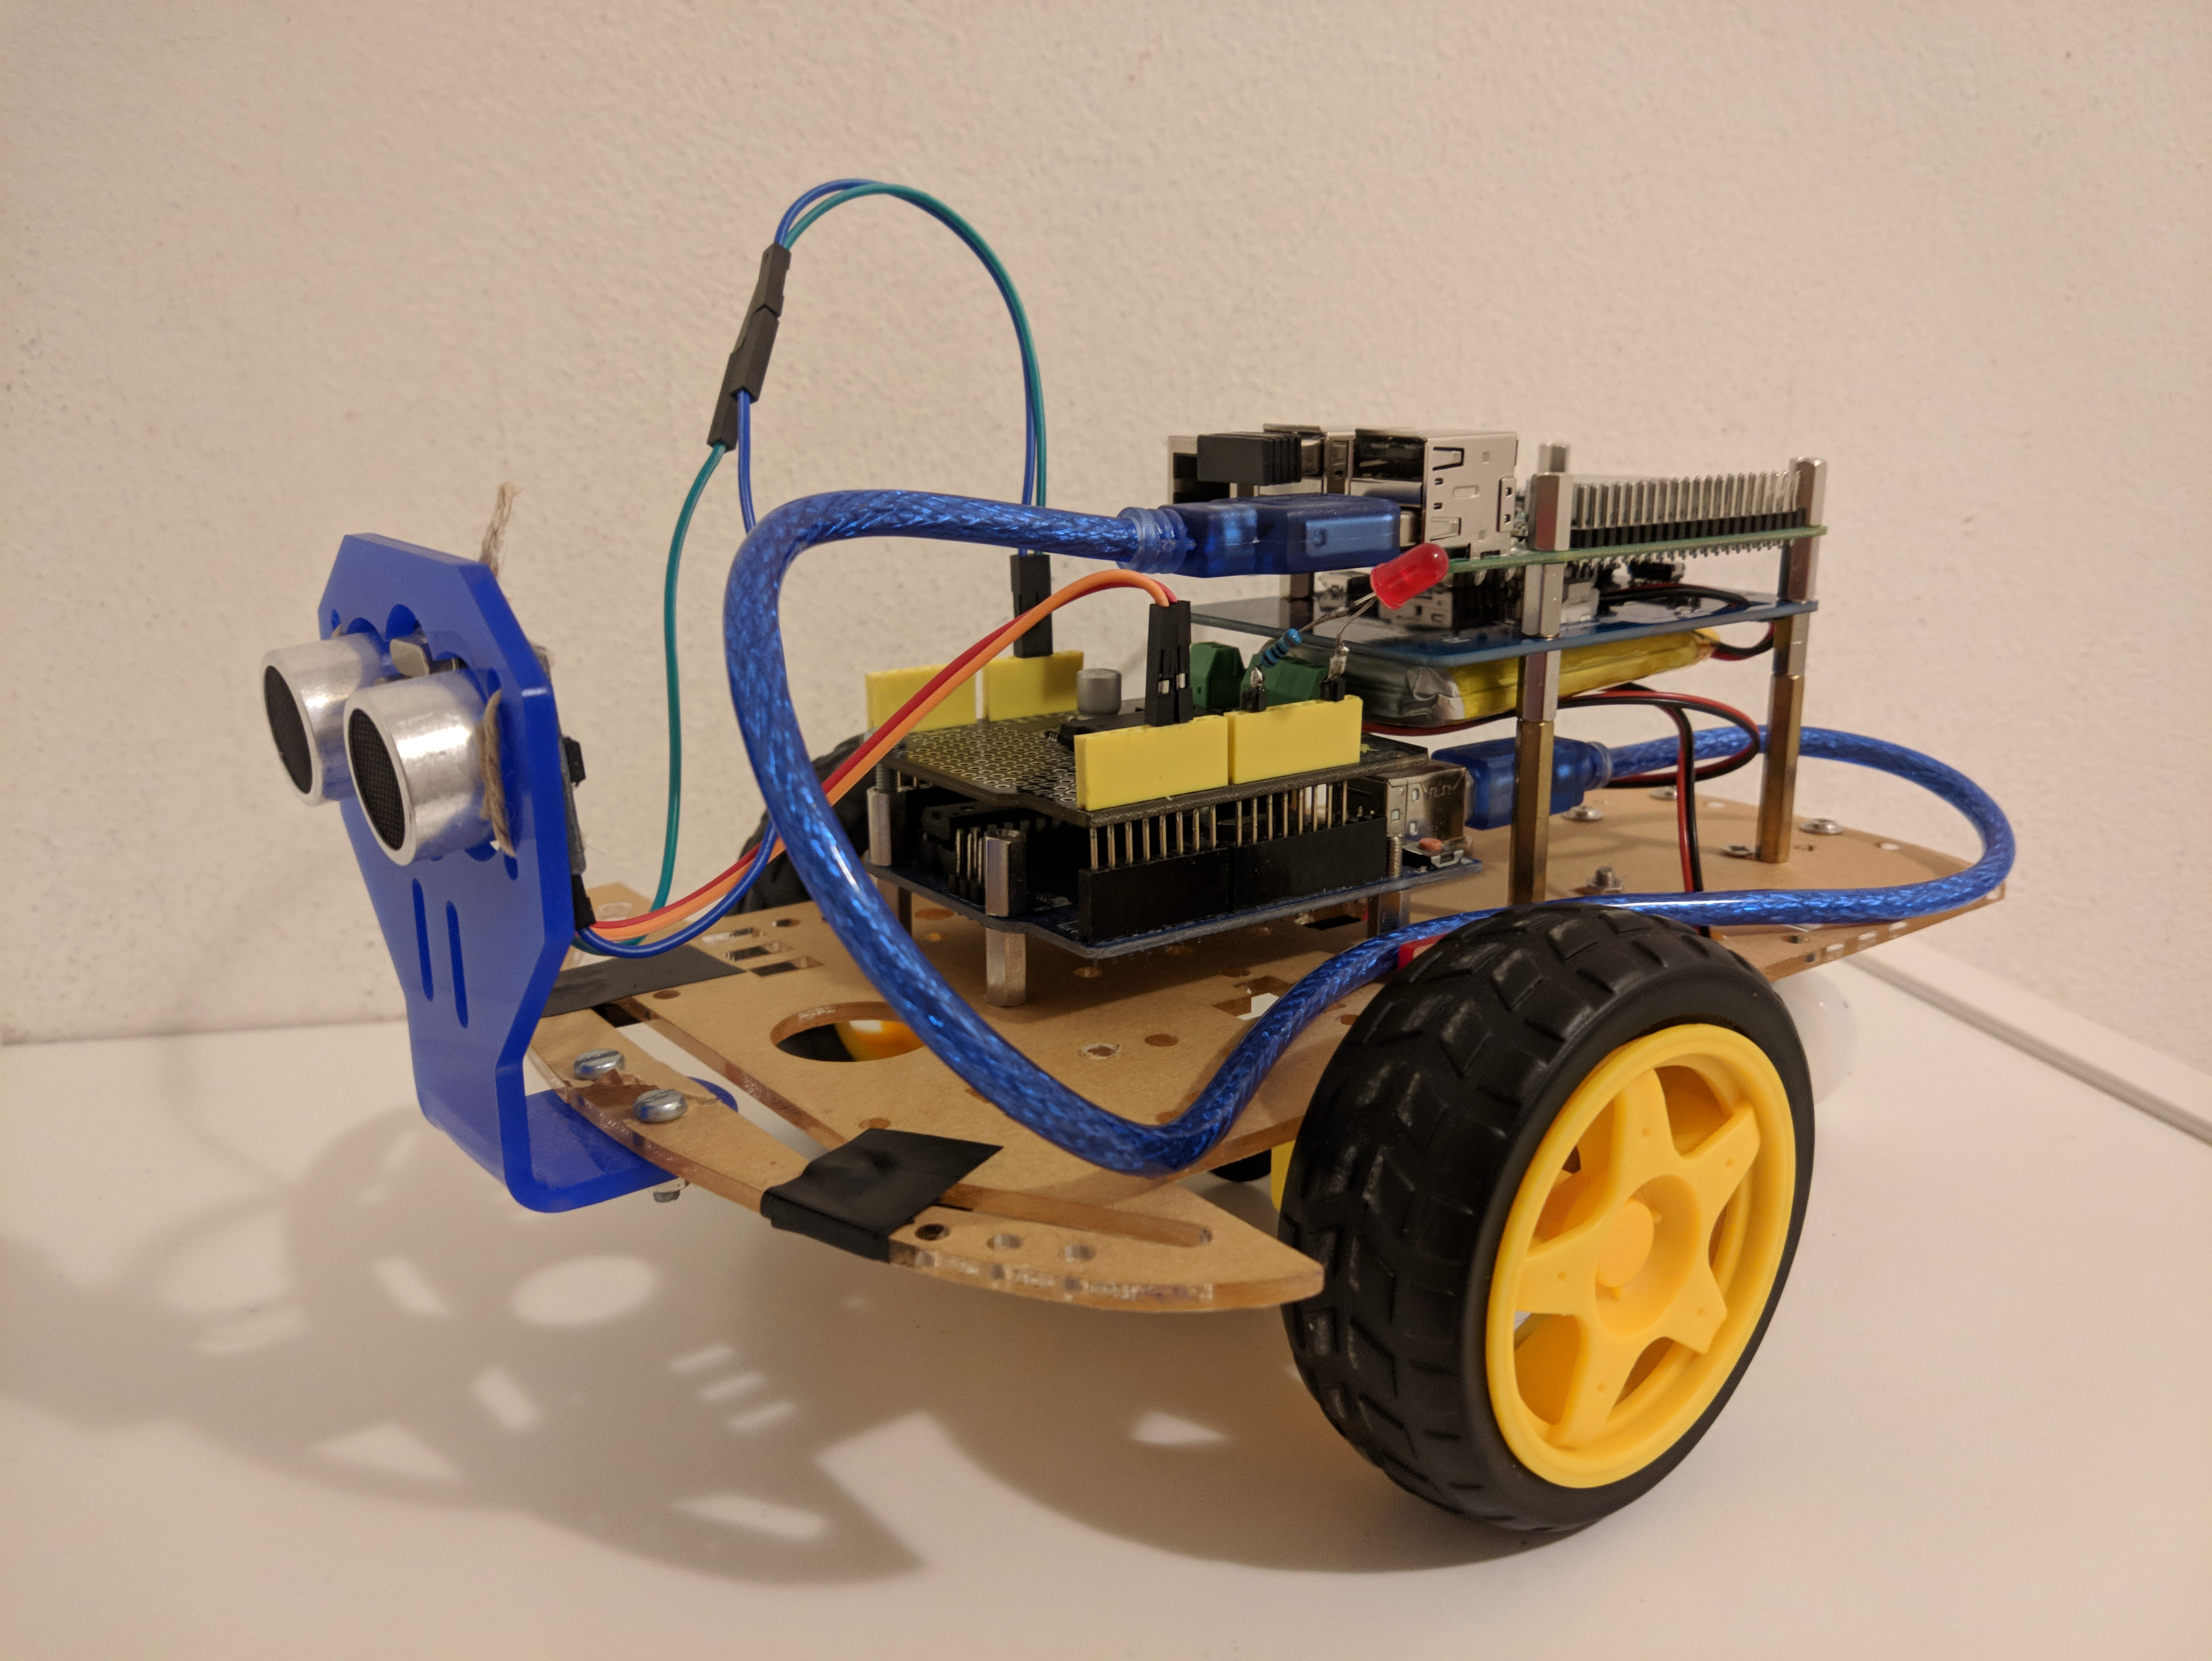
\includegraphics[width=0.8\textwidth]{res/sprint4/robot-angle.jpg}%
  \caption{Robot realizzato con Raspberry Pi e Arduino Uno}%
  \label{fig:sp4:robot-hw}
\end{figure}

\subsubsection{Trasmissione e memorizzazione delle foto}

Dal momento che le informazioni scambiate tra robot-console-interfaccia sono di tipo testuale, si è dovuto valutare un \textbf{sistema per la codifica delle immagini} in maniera testuale per il loro invio.

Una possibilità poteva essere quella di memorizzare le immagini nel robot stesso e inviare solamente l'indirizzo per il loro accesso.
Questo approccio però non rispettava pienamente i requisiti del sistema (dove si chiede esplicitamente di inviare le foto e la loro memorizzazione viene fatta sulla console), inoltre aumentava il livello di centralizzazione del sistema ed appesantiva ulteriormente la parte più sensibile: il robot.

L'approccio alternativo, che poi è quello che si è scelto di adottare, consiste nel codificare l'immagine in \textbf{Base64} dal robot per poi inviarla alla console che si occuperà di gestire questa informazione inserendola nello stato ed inoltrandolo alle interfacce tramite MQTT\@.

Per quanto riguarda il formato di memorizzazione, il committente non ha espresso preferenze, quindi si è deciso di salvare una foto ed un file testuale contenete le informazioni di contesto.

\section{Sprint Review}

Terminata la realizzazione del sistema, è stata effettuata l'ultima Sprint Review con il committente per la risoluzione delle ultime problematiche e l'analisi di quanto realizzato.

Le problematiche di lancio dell'applicativo Java sul robot fisico sono state risolte ed è stato richiesto un documento aggiuntivo che riassumesse in modo meno dettagliato il processo di sviluppo, focalizzandosi soprattutto su quanto sia cambiato tra la fase di analisi e quella di progetto, includendo schemi simili a quello in~\Cref{fig:sp4:system}.
Il documento \texttt{summary.pdf} prodotto è disponibile sul repository GitHub di questo progetto.
